\documentclass{article}
\input{imports.tex}
\input{config.tex}

\begin{document}
\noindent \textbf{MA3701 Optimización}\\
\textbf{Profesor:} Alejandro Jofré\\
\textbf{Auxiliar:} Benjamín Vera Vera

\begin{center}
    \Huge{\textbf{Examen}}\\
\textit{\large{Tiempo: 3:00}}\\
    \normalsize
    9 de diciembre de 2025
\end{center}
\begin{enumerate}
	\item Considere el siguiente problema de optimización:
		\begin{align*}
			\min_{x, y} \; & (x + y - 6)^2  \\
				       & x^2 + y^2 = 1.
		\end{align*}
		\begin{enumerate}
			\item Encuentre todos los puntos críticos de este problema.
			\item Utilice la condición suficiente de segundo orden para decidir cuáles de los puntos críticos obtenidos son mínimos locales del problema.
		\end{enumerate}
	\item Sea la función \(f : \mathbb{R}^n \to \mathbb{R}\) dada por
		\[
			f(x) = \sqrt{\norm{x}^2 + 1}.
		\]
		\begin{enumerate}
			\item Calcule \(\nabla f(x)\).
			\item Considere la regla de iteración por método de máximo descenso aplicada a \(f\) a partir de \(x_0 \neq 0\) y con paso \(\alpha\). Encuentre una expresión analítica para la iteración siguiente \(x_{k+1}\) en términos de la iteración actual \(x_k\) y el paso escogido \(\alpha\).
			\item Utilizando lo anterior, encuentre una fórmula para \(\alpha^*_k\) el paso correspondiente a la búsqueda de línea exacta en la iteración \(k\).
		\end{enumerate}
	\item
		\begin{enumerate}
			\item Utilizando el algoritmo Simplex, resuelva el siguiente problema de optimización lineal:
\begin{alignat*}{3}
\max\;&\; & -2x_1 &\;-\;& x_2 \\
\text{s.a.}\quad
& & -x_1 &\;+\;& x_2 &\le -1,\\
& & -x_1 &\;-\;& 2x_2 &\le -2,\\
& & &\; & x_2 &\le 1,\\
& & x_1,\,x_2 &\ge & 0.
\end{alignat*}
Entregue los maximizadores \(x_1, x_2\) así como el valor óptimo del problema.
\item Utilice el algoritmo de Dijkstra para encontrar el camino más corto entre \(x_0\) y \(x_9\) en el grafo de la figura \ref{fig:graph}.
\begin{figure}[htbp]
	\centering
	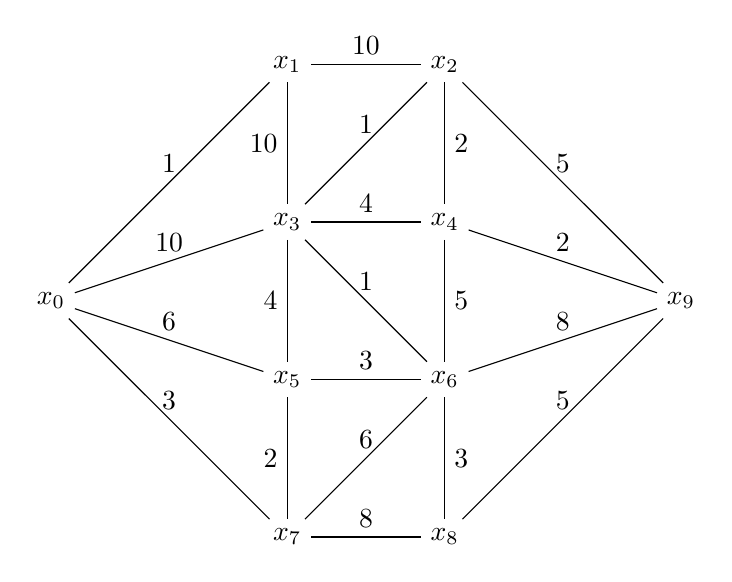
\begin{tikzpicture}
		\node (x0) at (-4, 0) {\(x_0\)};
		\node (x1) at (-1, 3) {\(x_1\)};
		\node (x2) at ( 1, 3) {\(x_2\)};
		\node (x3) at (-1, 1) {\(x_3\)};
		\node (x4) at ( 1, 1) {\(x_4\)};
		\node (x5) at (-1,-1) {\(x_5\)};
		\node (x6) at ( 1,-1) {\(x_6\)};
		\node (x7) at (-1,-3) {\(x_7\)};
		\node (x8) at (1, -3) {\(x_8\)};
		\node (x9) at ( 4, 0) {\(x_9\)};

		\draw[-] (x0) -- node[midway, above] {1}  (x1);
		\draw[-] (x0) -- node[midway, above] {10} (x3);
		\draw[-] (x0) -- node[midway, above] {6}  (x5);
		\draw[-] (x0) -- node[midway, above] {3}  (x7);
		\draw[-] (x1) -- node[midway, left]  {10} (x3);
		\draw[-] (x3) -- node[midway, left]  {4}  (x5);
		\draw[-] (x5) -- node[midway, left]  {2}  (x7);
		\draw[-] (x1) -- node[midway, above] {10} (x2);
		\draw[-] (x3) -- node[midway, above] {1}  (x2);
		\draw[-] (x3) -- node[midway, above] {4}  (x4);
		\draw[-] (x2) -- node[midway, right] {2}  (x4);
		\draw[-] (x3) -- node[midway, above] {1}  (x6);
		\draw[-] (x5) -- node[midway, above] {3}  (x6);
		\draw[-] (x4) -- node[midway, right] {5}  (x6);
		\draw[-] (x7) -- node[midway, above] {6}  (x6);
		\draw[-] (x7) -- node[midway, above] {8}  (x8);
		\draw[-] (x6) -- node[midway, right] {3}  (x8);
		\draw[-] (x2) -- node[midway, above] {5}  (x9);
		\draw[-] (x4) -- node[midway, above] {2}  (x9);
		\draw[-] (x6) -- node[midway, above] {8}  (x9);
		\draw[-] (x8) -- node[midway, above] {5}  (x9);
	\end{tikzpicture}

	\caption{Grafo pregunta 3}\label{fig:graph}
\end{figure}
	
		\end{enumerate}
\end{enumerate}

\end{document}
